% Generator: hand-authored TikZ from the source-visible axes, segment, and labels.
% Source: src-b46bf909434f6686413681f206c6f1c3566760d6e574f4799dc8b1e0658f9ee8
% PDF SHA-256: b798af61afdac624589769db5bbafe734aa9a0016973bd00b3f5bc8028ab3a40
% PDF page 1, printed page 70, question 8. Only the printed segment and labels are shown.
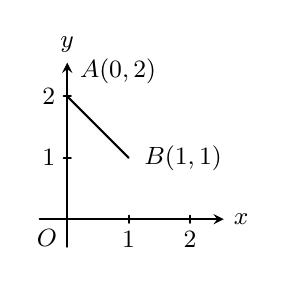
\begin{tikzpicture}[x=0.78cm,y=0.78cm,line cap=round,line join=round,line width=0.65pt,>=stealth,font=\small]
  \draw[->] (-0.45,0) -- (2.55,0) node[right] {$x$};
  \draw[->] (0,-0.45) -- (0,2.55) node[above] {$y$};
  \draw (-0.06,1) -- (0.06,1) node[left=2pt] {$1$};
  \draw (-0.06,2) -- (0.06,2) node[left=2pt] {$2$};
  \draw (1,-0.06) -- (1,0.06) node[below=2pt] {$1$};
  \draw (2,-0.06) -- (2,0.06) node[below=2pt] {$2$};
  \node[below left] at (0,0) {$O$};
  \draw[thick] (0,2) -- (1,1);
  \node[above right=1pt] at (0,2) {$A(0,2)$};
  \node[right=2pt] at (1,1) {$B(1,1)$};
\end{tikzpicture}
